
\subsection{Mesh Denoising}
\label{subsec:L0 denoising}

Different from denoising in point cloud, for mesh surfaces, there are vertex connectivity and triangle quality that can be used or considered.
But how to distinguish features from noise is still a challenging problem. 

\paragraph{(1)}
In image processing, \cite{xu2011image}, aiming to smooth images, provides an algorithm for directly optimizing the $\ell_0$ norm of gradients of image colors to create piecewise constant images.
Let $\mathbf{c}$ be a vector of pixel colors and $\triangledown \mathbf{c}$ be a vector of gradients of these colors.
They formulates the smooth problem as

\small{
\begin{equation}
 \label{eq:imagesmooth}
 \min_{\mathbf{c}}|\mathbf{c}-\mathbf{c}^{*}|^2+|\triangledown \mathbf{c}|_0
\end{equation}
}
\\
where $\mathbf{c}^{*}$ represents the original image colors to provide a data fidelity term.

A natural extension to triangulated meshes is to design a discrete differential operator to replace $\triangledown c$ that is zero when the surface is flat for arbitrary triangulations irrespective of the rotation or translation of the surface.
This constraint implies that some form of second order information rather than the first order information provided by $\triangledown c$ is needed, e.g.,  the discrete Laplacian operator\cite{pinkall1993computing} which is computed as a weighted combination of a vertex and its one-ring where the weights are given by cotangents of angles of the triangles.
However,
\parpic[r]{\label{fig:failureLaplaciandenoise}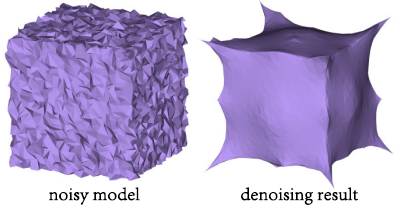
\includegraphics[width=0.4\linewidth]{images/denoise12}}
the vertex-based Laplacian only constrains the mean curvature vector as opposed to a metric that should directly measure sharpness per edge, then the optimization fails to reproduce sharp features well shown as the right figure.

\parpic[r]{\label{fig:edgeoperator}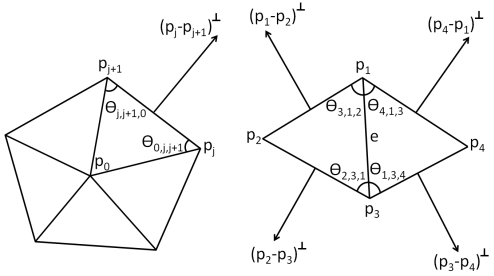
\includegraphics[width=0.5\linewidth]{images/denoise11}}
\cite{he2013mesh} generalizes this construction of the vertex-based cotan operator to an operator that acts directly on an edge

\small{
\begin{equation}
 \label{eq:edgecotanoperator}
 D(e) := {\left[ \begin{array}{c}
 \frac{\vartriangle_{1,2,3}((p_4-p_3)\cdot(p_3-p_1))}{\vartriangle_{1,3,4}((p_1-p_3)\cdot(p_3-p_2))} \\
 \frac{\vartriangle_{1,3,4}}{\vartriangle_{1,2,3}+\vartriangle_{1,3,4}} \\
 \frac{\vartriangle_{1,2,3}((p_3-p_1)\cdot(p_1-p_4))}{\vartriangle_{1,3,4}((p_2-p_1)\cdot(p_1-p_3))} \\
 \frac{\vartriangle_{1,2,3}}{\vartriangle_{1,2,3}+\vartriangle_{1,3,4}}
 \end{array}
 \right]}^{T}
 \left[ \begin{array}{c}
 p_1 \\ p_2 \\ p_3 \\ p_4
 \end{array}
 \right]
\end{equation}
}

Then the extended optimization problem is to make the edge operator sparse formulated as following

\small{
\begin{equation}
 \label{eq:L0 denoise}
 \min_{p,\delta}|p-p^{*}|^2+\alpha|R(p)|^2+\beta|D(p)-\delta|^2+\lambda|\delta|_0
\end{equation}
}
\\
where $p$ are the vertices of the shape, $p^{*}$ are their initial positions, $D(p)$ is a vector where the $i^{th}$ entry corresponds to the area-based edge operator applied to the $i^{th}$ edge, and $R(p)$ is a regularization term. Figure~\ref{fig:L0 denoise}gives one denoised result with sharp features.

\begin{figure}[ht]
  \centering
  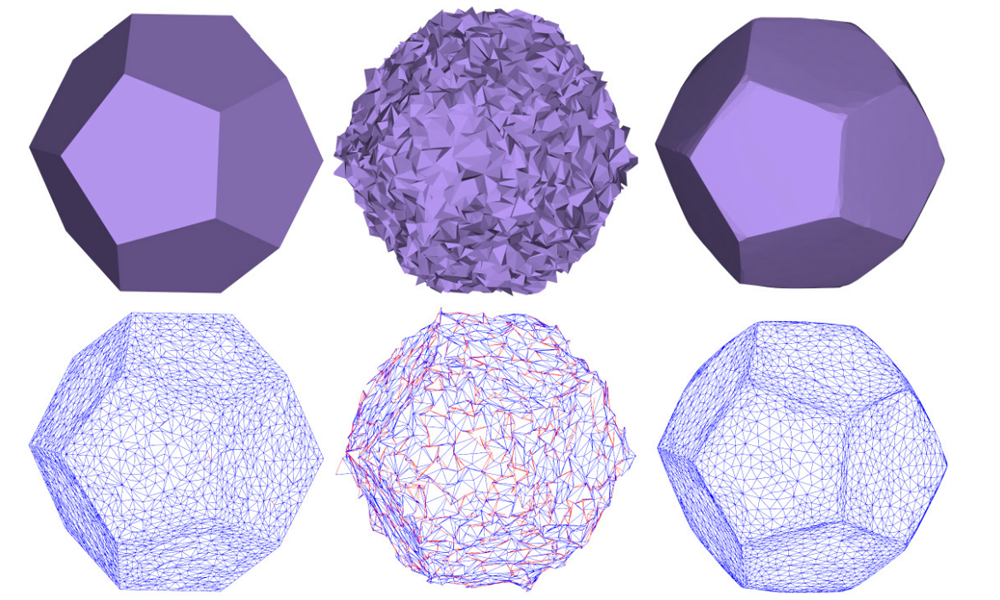
\includegraphics[width=2.5in]{images/denoise1}
  \caption{Sparse regularization: mesh denoising\cite{he2013mesh}. Left: initial surface. Center: surface corrupted by Gaussian noise in random directions with standard deviation $\sigma=0.4l_{e}$($l_{e}$ is the mean edge length). Right: denoising result. The wireframe shows folded triangles as red edges.}
  \label{fig:L0 denoise}
\end{figure}

\begin{figure*}[ht]
  \centering
  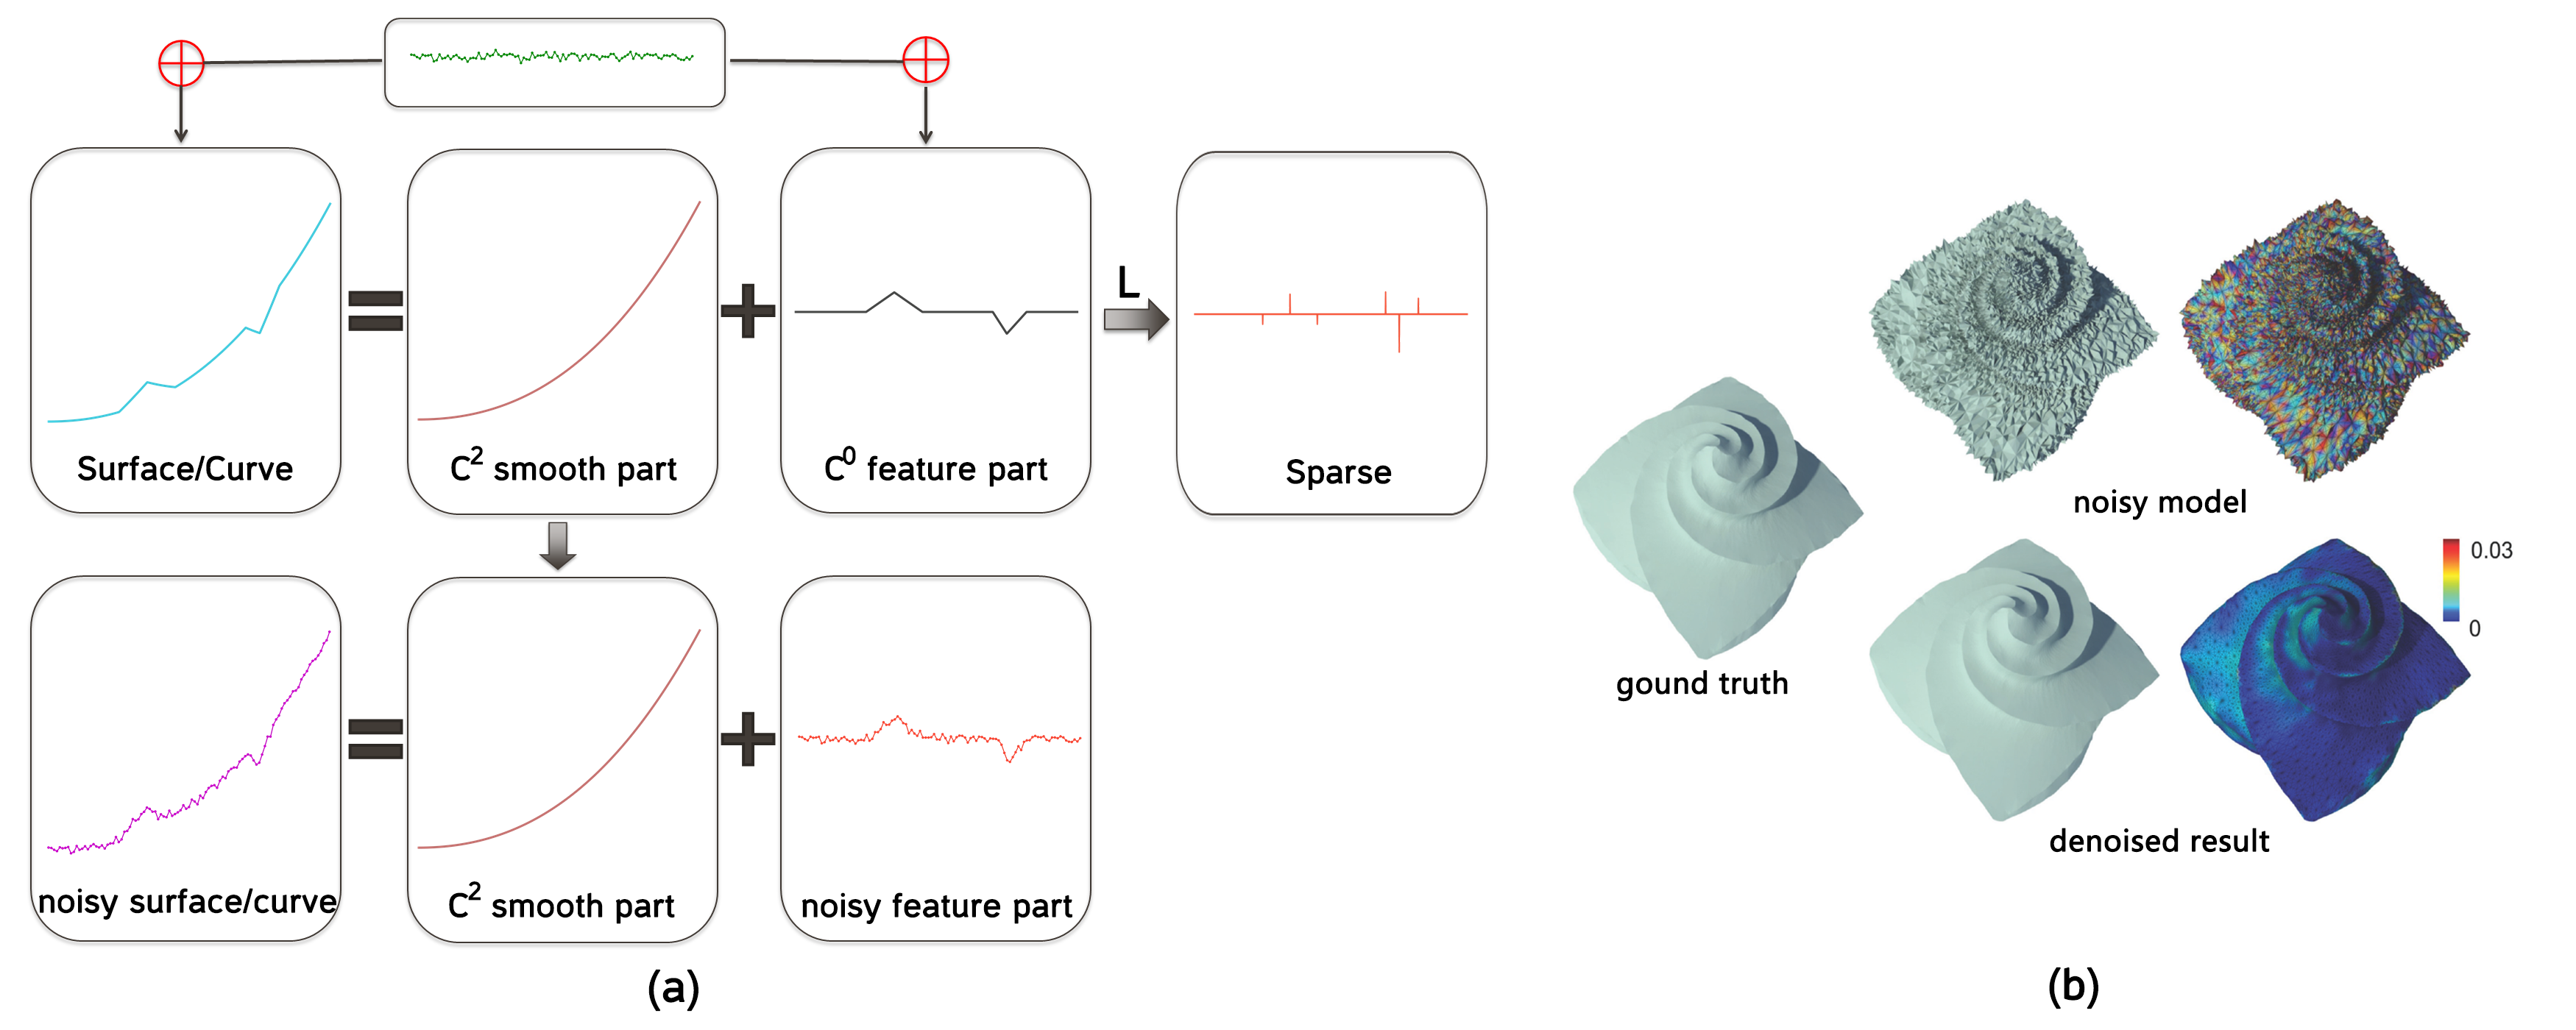
\includegraphics[width=5in]{images/denoise2_1}
  \caption{Sparse regularization: mesh denoising\cite{wang2014decoupling}. (a) is the two-dimensional illustration for their key observation. (b) is a denoising example.}
  \label{fig:decoupling}
\end{figure*}

\paragraph{(2)}
Like most previous methods, how to tune the parameters shown in~(\ref{eq:L0 denoise}) has not theoretical guarantee and the computation of differential properties for distinguishing noise from feature is unreliable and unstable.

To address these problems, \cite{wang2014decoupling} presents a two-phase approach for decoupling features and noise on discrete surfaces.
Figure~\ref{fig:decoupling}(a) gives a two-dimensional curve as the illustration for their key observation: any surface is piecewise $C^2$, that is, a surface consists of two parts: $C^2$ smooth part and $C^0$ feature part which can be transformed into a sparse signal by applying the Laplacian operator.
As such, the denoising problem is divided into two phase: smooth part(base mesh) estimation and recovering features from the corrupted feature part.

They firstly get a base mesh by denoising the input data using a global Laplacian regularization smoothing optimization, in which the smoothness parameter is automatically chosen by adopting the generalized cross-validation scheme,
then decouple the features $x$ and noises simultaneously from the noisy feature part $y$ via the $\ell_1$ analysis compressed sensing optimization

\small{
\begin{equation}
 \label{eq:decoupling}
 \min_{x}\|Lx\|_1~~ s.t. ~ \|y-x\|_2 \le \epsilon
\end{equation}
}

Finally, combining the denoised feature part and the obtained base mesh reduces the final denoising result. Note that it is the first time noise and features are analyzed and separated in such an elegant manner with guarantees by statistical theory which is much exciting and sightworthy in the smoothing optimization. 